\begin{frame}{Exmple Usage}
    \begin{columns}
        \begin{column}{.66\textwidth}
            Single pass of HSI:       
            $p\times q$ Internet Protocol Data:
            \begin{itemize}
                \item Time series parsing of the Carbon-Black Logs
                \item Preprocessing: Encoding, Scaling, and PCA
                \item HSI Inferences
                \item Multi-filtered
                \item Multi Filter Count
            \end{itemize}
        \end{column}
        \begin{column}{.33\textwidth}
            \bc
            \vspace{-.5in}
            \begin{figure}               
                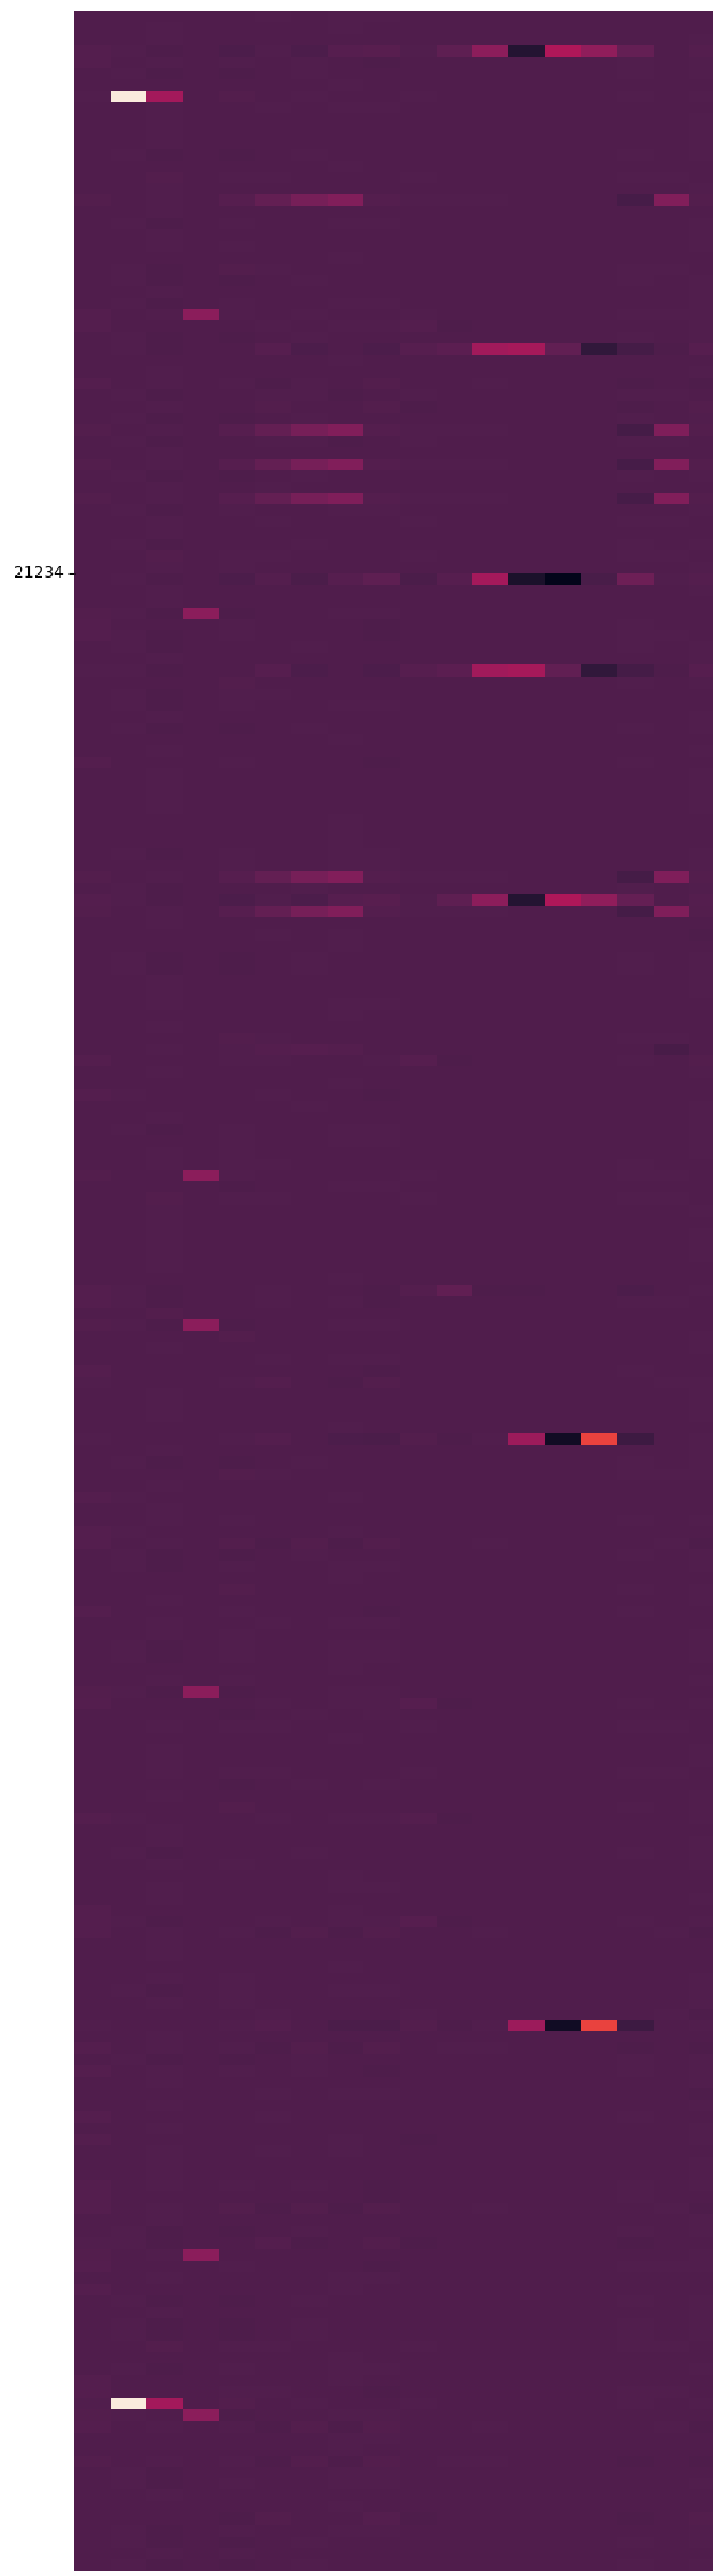
\includegraphics[height=.7\textheight]{../Images/model_pipeline_tikz/CyberPred/raw_data.pdf} 
            \caption{Preprocessed input data relevant to Cyber Security.}       
            \end{figure}
            \ec
        \end{column}
    \end{columns}
\end{frame}


\begin{frame}{Exmple Usage}
    \begin{columns}
        \begin{column}{.66\textwidth}
            Single pass of HSI:       
            $p\times q$ Internet Protocol Data:
            \begin{itemize}
                \item Time series parsing of the Carbon-Black Logs
                \item Preprocessing: Encoding, Scaling, and PCA
                \item HSI Inferences
                \item Multi-filtered
                \item Multi Filter Count
            \end{itemize}
        \end{column}
        \begin{column}{.33\textwidth}
            \bc
            \vspace{-.5in}
            \begin{figure}               
                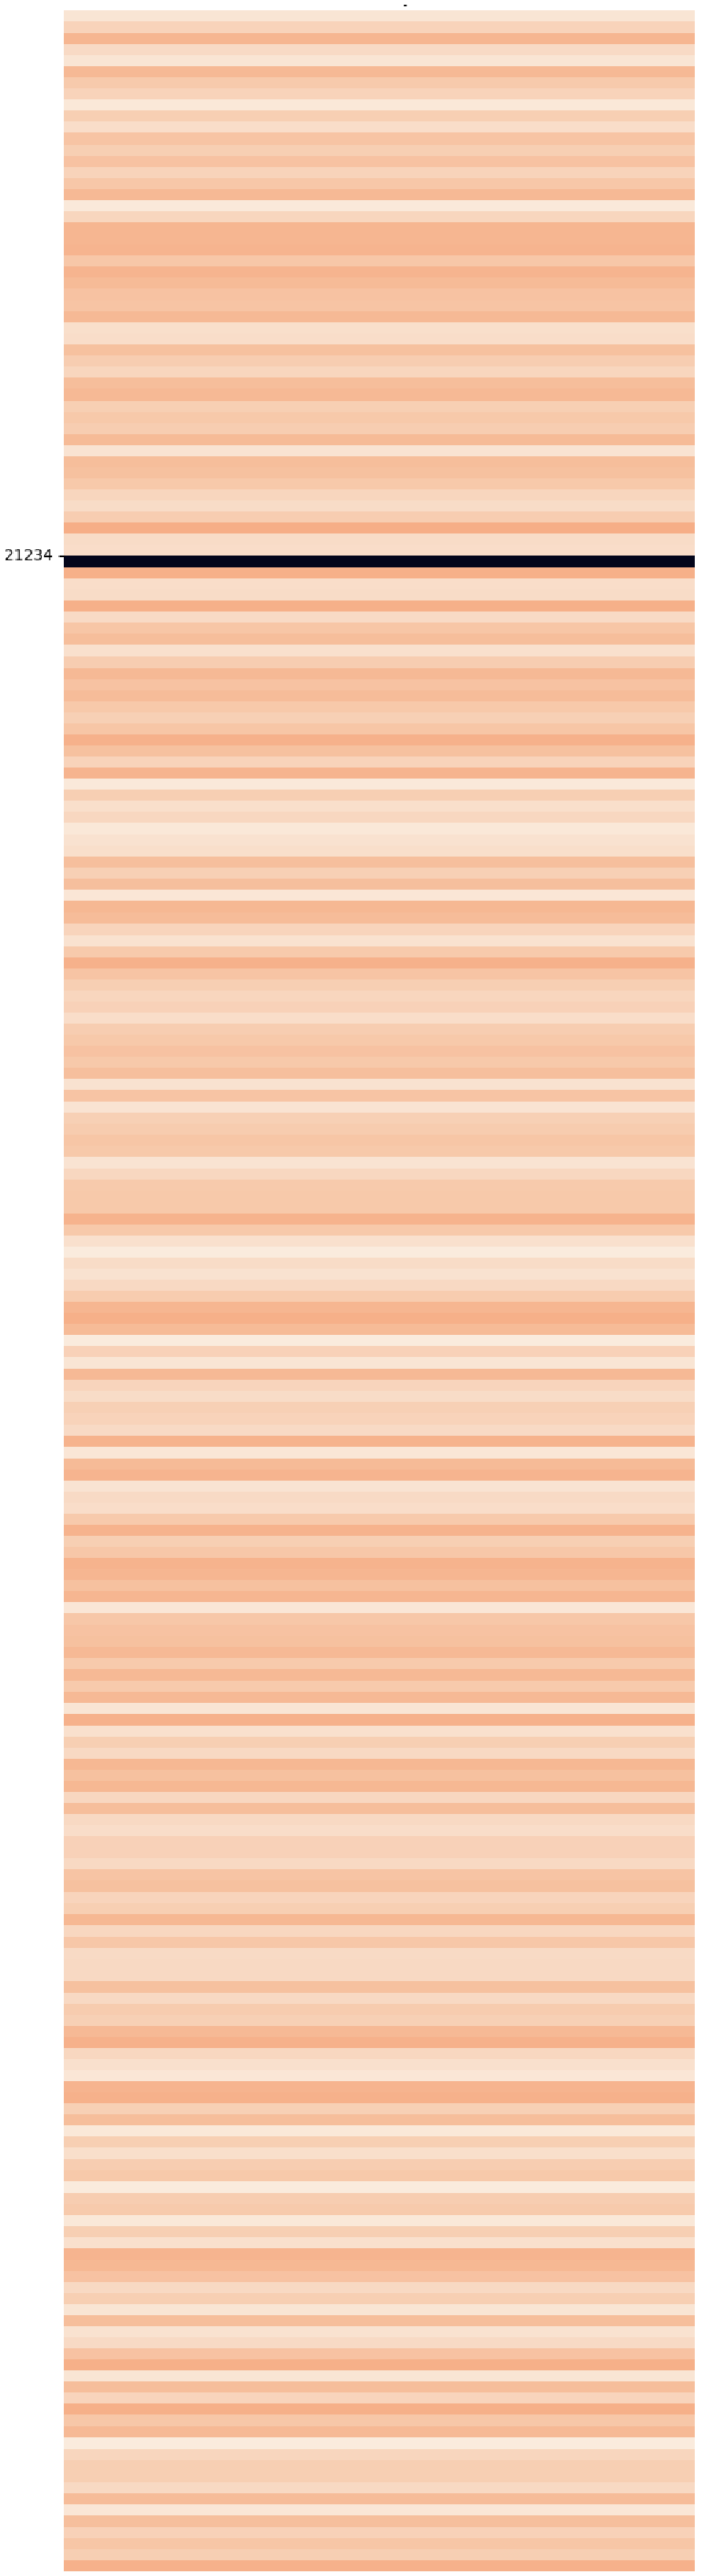
\includegraphics[height=.7\textheight]{../Images/model_pipeline_tikz/CyberPred/anomaly_score.pdf} 
            \caption{Multi-filter count after 15 filters. Max value of 13. }       
            \end{figure}
            \ec
        \end{column}
    \end{columns}
\end{frame}


\begin{frame}{Exmple Usage}
    \begin{columns}
        \begin{column}{.66\textwidth}
            Multi-filtered HSI:       
            $p\times q$ Internet Protocol Data:
            \begin{itemize}
                \item Time series parsing of the Carbon-Black Logs
                \item Preprocessing: Encoding, Scaling, and PCA
                \item HSI Inferences
                \item Multi-filtered
                \item Multi Filter Count
            \end{itemize}
        \end{column}
        \begin{column}{.33\textwidth}
            \bc
            \vspace{-.5in}
            \begin{figure}               
                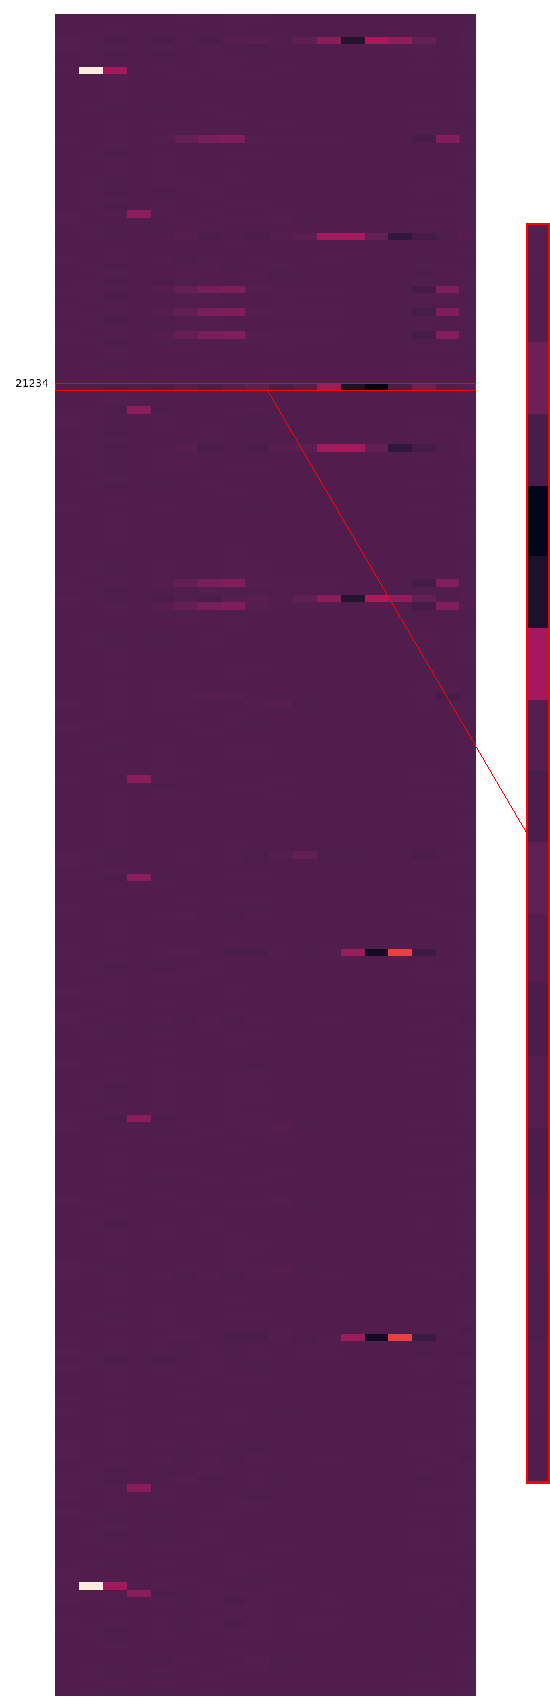
\includegraphics[height=.7\textheight]{../Images/model_pipeline_tikz/CyberPred/anomaly_raw_data.pdf} 
            \caption{Anomalous data point predicted by the HSI model. }       
            \end{figure}
            \ec
        \end{column}
    \end{columns}
\end{frame}
